%Written Report
%The report should be single-column, single-spaced, with 1” margins and appropriate section headings, written in Word (11pt Arial or 12pt Times New Roman font) or LaTeX (11pt Computer Modern or 12pt Times font). It should
%be at least two and not more than four pages long, not counting the title page and unlimited space for figures and
%references. It must include a title page consisting of the report title, student name, research advisor (if applicable),
%an abstract of at most 150 words, and full bibliographic information about the selected paper. The title of the
%report should describe the topic of the critical analysis presented therein and thus should be different from the
%title of the paper. It is essential to adhere to scholarly standards with regard to plagiarism. Duplication of figures
%may be appropriate and must be accompanied by a suitable citation. Lengthy quotations are generally
%inappropriate. If equations or algorithms are duplicated from the paper, the surrounding text should make this
%clear. Students should assume that the examination committee members have read the selected paper and should
%summarize accordingly. The purpose of the report is not to repeat the contents of the selected paper, but rather
%to provide a critical assessment.
%
%The following organization is recommended for the report:
%• Summary of the problem (about 1/2 page): What problem is addressed in the paper? What was the state
%of the art in the field related to this problem? Is the problem important, and why? (Unless the arguments
%for why a problem is unimportant are novel and compelling, it is generally disadvantageous to select a paper
%that addresses an unimportant problem.)
%• Key ideas and main innovation (about 1/2 page): What innovation is presented in the paper? Explain the
%concept, i.e. how it works, in some detail, and how it represents an advance over previous knowledge.
%• Critique (about 1 page): What are the strengths and weaknesses of the innovation in the present paper
%relative to other approaches? Read references and search to understand the field. Coverage of alternative
%approaches need not be exhaustive, but a command of principal alternatives should be demonstrated.
%• Suggestions for improvement or future work (about 1 page): Propose at least one further line of research in
%the field based on analysis of the current paper and the insights gained from it. Students must be able to
%support proposed ideas with rational arguments. Having preliminary results is encouraged but is not
%required.
%In addition, the report should adhere to the following guidelines:
%• Use of figures: Figures should be numbered in the order in which they are discussed in the report. Figure
%captions should clearly explain the content and importance of the figures. The caption should indicate
%whether the figure is original or a reproduction; if it is a reproduction, the source should be clearly cited.
%• Use of references: The report should cite appropriate prior works to substantiate any arguments or claims
%made in the report. It should contain a minimum of 5 references. The bibliography should be in IEEE style
%or in any other verbose style appropriate to the student’s subdiscipline.

% PREAMBLE
\documentclass{article}
\usepackage[letterpaper, margin=1in]{geometry}
\usepackage{graphicx}
\usepackage[style=numeric-comp]{biblatex}
\usepackage{color}

\addbibresource{./assets/sources.bib}
\newcommand{\todo}[1]{\textbf{\color{red}#1}}
\newcommand{\citationneeded}{\textbf{\color{blue}[Citation Needed]}}
\begin{document}
\begin{titlepage}
   \begin{center}
       \vspace*{1cm}

       \textbf{A Review of Motions in Microseconds}

       %\vspace{0.5cm}
       % Thesis Subtitle
            
       \vspace{1.5cm}

       \textbf{Student Name: Pravi Samaratunga}

       \textbf{Advisor Name: Sabrina Neuman}

       \vfill
            
       \vspace{0.8cm}
            
       Boston University\\
       Electrical and Computer Engineering\\
       \today

       \vspace{3cm}
     
       
\includegraphics[width=0.4\textwidth]{./assets/BU_logo.png}
            
   \end{center}
\end{titlepage}

\todo{Big Todos: \begin{itemize}\item Some phrasing may match MiM a little too closely; run through plagiarism checker. \item Replace \citationneeded with actual citations.\item Abstract (150 wd max)\end{itemize}}

\section{Introduction}

Sampling-based motion planners have computationally expensive subroutines, including collision checking, nearest neighbors search, and forward kinematics. By improving the performance of some of these planning primitives, sampling-based motion planners can acheive substantial improvements. Sampling-based motion planners are commonly used in robotics, and speedups in this domain can improve safety and responsiveness. Motion planning for robotic manipulation tasks often takes several seconds to execute\citationneeded. If motion planning can be done on the fly, the ability to plan reactively could expose whole problem domains that were previously impractical to explore. %Domestic applications such as cooking are now possible. \todo{Ask Radhika about what those problem domains are.}

By using the architectural principles of fine-grained parallelism and work-ordering, the researchers were able to achieve a 500x speedup over previous state-of-the-art approaches.

\subsection{Planning Primitives}

Sampling based motion planning (\textsc{sbmp}) algorithms such as \textsc{rrt}, \textsc{prm}, and \textsc{est} \citationneeded can all be broken down into several common steps. They must all sample the state space, building a state tree to explore. This typically makes use of a \textit{nearest neighbors} (\textsc{nn}) search of the state space. The state is mapped to physical space using \textit{forward kinematics} (\textsc{fk}). The planner next \textit{checks for collisions} (\textsc{cc}) to ensure that the selected state does not collide with any obstacles in the environment, nor does any point in the state space along the edge that is added. This is conventionally thought to be the most computationally intensive step of the process \citationneeded. 

\todo{I'm poking through the cited Choset etal but not finding an explicit breakdown of planning primitives like above. I'm not entirely sure this is exhaustive.}

\todo{I don't refer to Motion Validation by name. Is that a problem?}

\subsection{State of the Art}

Collision checks are performed in two sweeps: \textit{broadphase} and \textit{narrowphase}. Broadphase approximates a set of possible collisions by modeling the environment in faster-to-compute ways. Narrowphase takes these possible collisions and returns the actual collisions.
Historically, \textsc{sbmp} has been parallelized in a coarse-grained fashion, running many independent planners in parallel. There is space to optimize \textsc{sbmp} parallelism in terms of the planning primitives the authors identified. 

\section{Innovation}

In the paper, the authors present Vector Accelerated Motion Planning (\textsc{vamp}), which provides significant motion planning speedups by conceptualizing sampling-based motion planning as a composition of primitives, and introducing vectorized implementations of those primitives. Vectorizing these operations allows for fine-grained parallelism at the instruction level, which is underexplored in the robotics domain.

One of the major innovations presented is the use of a \textit{Struct-of-Arrays}, as opposed to the more traditional \textit{Array-of-Structs}. Figure \ref{fig:soa_aos} shows the difference in memory layouts between these two approaches.

\begin{figure}[h]

\label{fig:soa_aos}
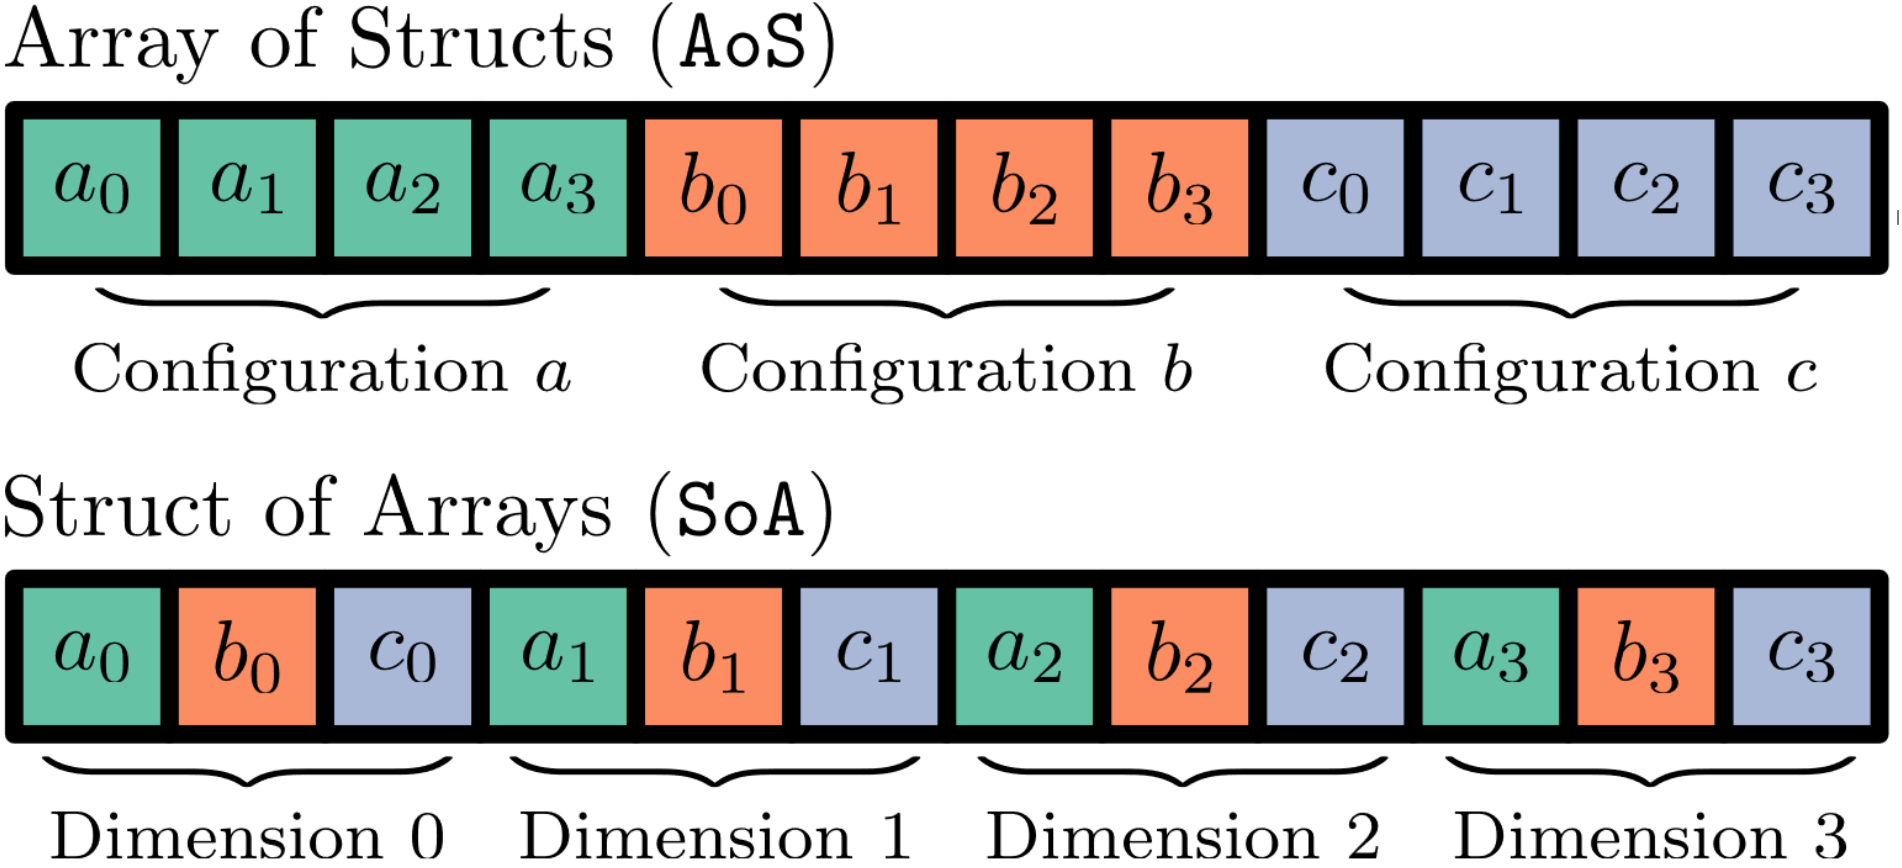
\includegraphics[width=0.8\textwidth]{./assets/soa_aos.png}

\caption{Figure duplicated from \citationneeded. This shows the difference between the Array-of-Structs (\textsc{AoS}) and Struct-of-Arrays (\textsc{SoA}) memory layouts. The latter is more amenable to \textsc{simd}} instructions.

\end{figure}

Due to CPU memory access patterns, the Struct-of-Arrays layout is more favorable for SIMD approaches. \textsc{vamp} replaces the existing \textsc{cc} \& \textsc{fk} primitives with vector-oriented versions, reducing the cost of given computation. 
In order to vectorize \textsc{fk}, \textsc{vamp} generates a \textit{trace} from a URDF to create an unrolled loop. 
In order to vectorize \textsc{cc}, the robots and obstacles are represented as a composition of bounding volumes (e.g. spheres), and collisions are calculated between these known geometries.

\todo{do more discussion of what vectorizing FK and CC entail}

\todo{discuss raked motion validator}

\section{Strengths \& Weaknesses}

This paper shows how some simple optimizations can yield serious empirical results, including a 500x speedup over the state of the art. However, the authors  pose the question of \textit{why} they get these results. They combine several innovations, but it remains unclear how each impacts end to end performance.

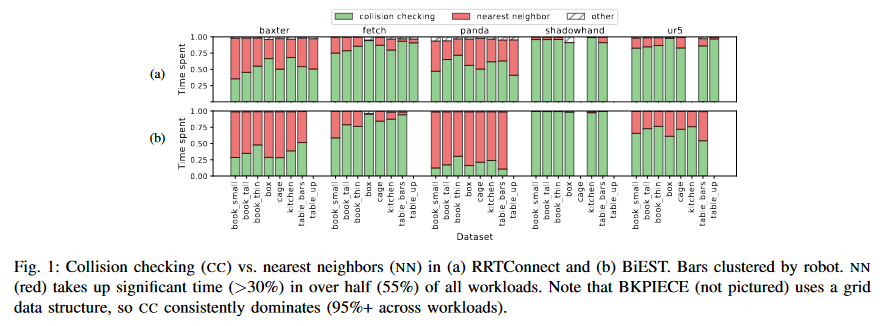
\includegraphics[width=0.8\textwidth]{./assets/cc_nn.png}

\todo{And here's some breakdown of that}

The paper also does not include much exploration on why different workloads show different amounts of improvement with the \textsc{vamp} optimizations. There’s less of a speedup in the 8DOF Fetch robot than the 7DOF Panda, though the speedup still very significant. \todo{Explicitly state those ratios - redo the entire table actually}

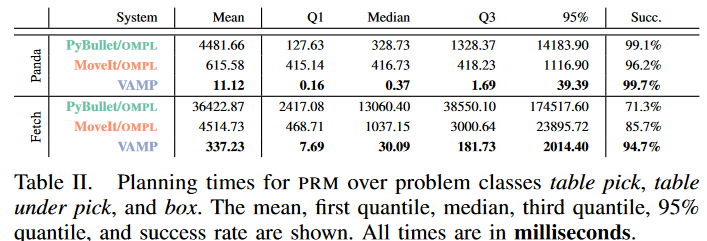
\includegraphics[width=0.8\textwidth]{./assets/78_table.png} \citationneeded

\section{Future Work}

I want to explore the particulars of the vectorized collision checking subroutine. While there is significant work in the trajectory optimization community using spheres as geometric primitives \citationneeded, there is research outside of the robotics domain regarding colliders using different kinds of geometric primitives, such as trimeshes and capsules \citationneeded \todo{see UE5 docs}. 

\end{document}